\documentclass[12pt]{report}
\usepackage[top=1.5cm, bottom=1.5cm, left=1cm, right=1cm]{geometry}
\usepackage[utf8]{inputenc}
\usepackage{amsmath}
\usepackage{amsfonts}
\usepackage{amssymb}
\usepackage{graphicx}
\usepackage{hyperref}
\usepackage{tcolorbox}
\usepackage{xcolor}
\usepackage{enumitem}
\usepackage{multicol}

\title{Computer Forensics and Cyber Crime Analysis}
\author{Alessandro Milani}
\date{\today}

\tcbset{
  sharp corners,
  colback = white,
  before skip = 0.2cm,    % add extra space before the box
  after skip = 0.5cm      % add extra space after the box
}                           % setting global options for tcolorbox

\definecolor{main}{HTML}{5989cf}    % setting main color to be used
\definecolor{sub}{HTML}{cde4ff}     % setting sub color to be used

\newtcolorbox{boxH}{
  colback = sub,
  colframe = main,
  boxrule = 0pt,
  leftrule = 6pt % left rule weight
}


\begin{document}

\maketitle

\tableofcontents

\part{Legal}
\chapter{Legal Introduction}

Beafore the technology was between us (classic telephon call), but with the advanced of the information technology,
the technology is now about us (facial recognition, social media, etc). \\
Example: The IA act say taht is not possible utilize IA for real time facial recognition without an "important" reason.\\
This generation use technology also for be profiled by an alghoritm for varius scope and not only for comunicate.   \\

The "technology was between us" was simpler and the only problem was to cehck if there is a conversetion and intercept it with a good quality.
Now, we have the problem of quantity. If we need to analyze data from milions of people we can end to vaiolate fundamental rights and make mistaks
(even with OSINT). \\
Surovieky theory: collective intelligence, the point is that if you have 10k persons say that the restuarant is good and only 10 that say it's a froud,
the collective intelligence say that the majority have right. In Forensics this can not be applied because you need to be 100\% secure of what you have.
(if in a trial you have only the 1\% that a person can't be guily you need to be in favor of him) [find better term]

In the technology in Us, and the advance of IA is important that the law split waht is uman and what is not (like be transparent when a content is AI gen and when not)

"Tesla case" whan there is an incident it need to understand in the percent of error that is from tesla and the percent from the partners.

\section{GDPR aand alghoritm bias}

Art.22 of GDPR, say that you always need to have human in the decision process

\section{Example - Lex Machina}
Tool that analyze all the legal case from a giurisdiction (like France) and classify
all the case in different categorys.
So if you have a case X in Paris with judge Y, you have 60\% possibility to win. If the Attorny ins Z, the probability is 80\%.

\section{Example - Compas}
alghoritm that help the jugde defice is the person can commit other crime or not
and so decide it need to stay in jail or get a reduce in the sentence (sconto della pena)

- A False positive in digital forensics can change people's lives.

%% 1. Introduction to the Course
%% 2. Foundations of Digital Forensics
%% 3. Cybercrime Convention
%% 4. Resolution Adopted by the UN General Assembly on 26 May 2021
%% 5. Garlasco case
%% 6. IoT and Digital Forensics
%% 7. Digital Forensics and Territorial Principle
%% 8. Remote Forensics: Hacking Team Case
%% 9. Digital Forensics and Artificial Intelligence
%% 10. The New Frontier of Digital Forensics in the AI Context
%% 11. Case studies and practical applications

\chapter{Foundations of Digital Forensics}

\section{Intro and definitions}

\subsection{Digital and Electronic Evidence}

By the Scientific Working Group on Digital Evidence (\textbf{SWGDE}) a definition of, 
\textbf{digital evidence} is "any information of evidential value 
whether memorized or sent in a digital format". It's used by the \textbf{Council of Europe} \\

Another definition come from the \textbf{ Eoghan Casey - 2004} that define 
a d\textbf{igital evidence or electronic evidence} as "any probative informationstored 
or transmitted in digital form that a party to a court case may use at trial". It's more related to the 
juridical part. \\

A last definition of \textbf{Electronic evidence} is information generated, stored or transmitted
using electronic devices that may be relied upon in court, defined by the 
\textbf{Council of Europe - 2013}. \\

\begin{boxH}
    For the exam, the first dfinition is the more important
\end{boxH}

So. in general, way we can say that a digital/electronic evidence need to be:
\begin{itemize}
    \item \textbf{invisible} to the untrained eye
    \item Need to be \textbf{interpreted} by a specialist
    \item It may be \textbf{altered} or \textbf{destroyed} through normal use
    \item It can be \textbf{copied} without limits
\end{itemize} 

\subsubsection{Legal Requirements}
The main characteristics that a Digital/Electronic Evidence need to have to be accepted in a trial are:
\begin{itemize}
    \item \textbf{Admissability:} it need to be compliant with law and best practices. \\ 
        What can be seen is not what can be admissed in court (ex. if the italian police enter in a laptop, 
        can only "wiretapping", by enabling mic and camera, 
        and can't use other information like email or files in court )
    \item \textbf{Authenticity:} avoid any digital evidence tampering
    \item \textbf{Reliability and believability:} readily understandable for a judge. \\
        If a judge not understand the evidence can ignore it
    \item \textbf{Proportionality:} respect fundamental rights of parties affected by the measure
\end{itemize}

\subsubsection{Find a digital evidence}
A digital evicence can be hidden in different place and a criminal usully use some classical ways 
(not the cloud becasue the access is easy form a pocile force)
like hidden folder, usb, extrnal memory etc.. can be hidden everywhere 

\subsubsection{Categories}
Three main types of digital evidence
\begin{itemize}
    \item \textbf{Created by human}: digital data result of an action taken by an human
    \begin{itemize}
        \item \textit{Human to Human}: Like an email
        \item \textit{Human to PC}: like a word document
    \end{itemize}
    \item \textbf{Created indipendenlty by the computer}: data that are result of 
    the processing of data by an algorithm and without human intervention
    \item \textbf{Created by both human and the computer}: somethings like a spreadsheet where the data 
    are entered by the human, and the result is worked out by the computer
\end{itemize}

\newpage
\subsubsection{Julie Amero Case}

\begin{boxH}
    This case is not import for the exam
\end{boxH}

Julie Amero is a supply teacher at Kelly School in Norwich, Connecticut
who was found guilty of showing pornography to children under the age of 16
for some popup that appear during a lesson

\begin{figure}[h!]
    \centering
    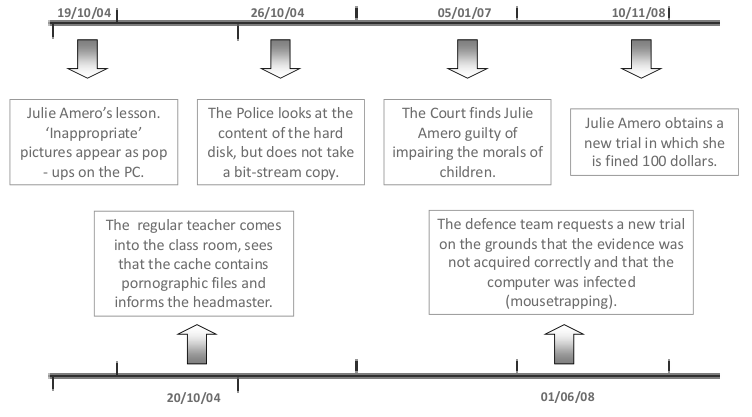
\includegraphics[width=1\textwidth]{img/amero_case.png}
    \caption{Timeline of the case}
    \label{fig:amero case}
 \end{figure}


\subsection{What is digital Forensics}

\textbf{Digital Forensics} is get hold of evidence without modifing the IT 
system in which that evidence is found, ensure that the 
evicence acuired in another medium is identical to the original and 
analyse data without modifyin it.

\subsection{The “Big Five” of Digital Forensics (Council of Europe)}

\begin{itemize}
    \item \textbf{Data Integrity:} No action taken \textit{should change electronic devices or media}, 
    which may subsequently be relied upon in court.
    \item \textbf{Chain of custody:} An \textit{audit trail} of all actions taken when handling electronic 
    evidence should be created and preserved
    \item \textbf{Specialist Support:} If investigations involving search and seizure of electronic 
    evidence it may be necessary to consult \textit{external specialists}. 
    \item \textbf{Appropriate Training:} First responders \textit{must be appropriately trained} to be able 
    to search for and seize electronic evidence if no experts are available at the scene
    \item \textbf{Legality:} The person and agency in charge of the case are responsible 
    for ensuring that \textit{the law and the above listed principles} are adhered to. 
\end{itemize}

\section{Digital Forensics Procedure}
Six phase of digital forensics procedure:

\subsection{Identify the Suspect}
There are 3 main phase for identify the suspect:

\begin{itemize}
    \item \textbf{Osint and Socmint:} Very usefull for collect information reguarding criminal 
    (even mafia ones), from social media, and other public sources.
    \item \textbf{Data Retension Directive in EU:} The investigator uses the Court 
    System to compel the ISP to reveal a physical location that 
    corresponds likely to the source of Network (IP Address)
    \item \textbf{Multiple User ID or multiple 
    Ips over time,  open Wi-Fi, Proxy, Botnet}: Under a warrant (depending from the Jurisdiction) 
    the location is searched and any computer or other device is seized
\end{itemize}

\subsubsection{Data Retension}
With the Directive 2006/24/EC, the EU member states are required to store data for 
a period of \textbf{6 to 24 months} (but can change from state to state). 
The data stored are gerally call detail records (CDR) of 
telephony and internet traffic and location data (IPDRs). \\
So evert single country and ISP have different data retention policy, and 
this can be a problem for the investigator, but from a privacy point of view a short time 
or null data retention is better.

\newpage

\paragraph{Transparency report:} Every year the ISP need to publish a transparency report 
where they show the number of request of data retention and the number of request that they 
have accepted.

\begin{figure}[h!]
    \centering
    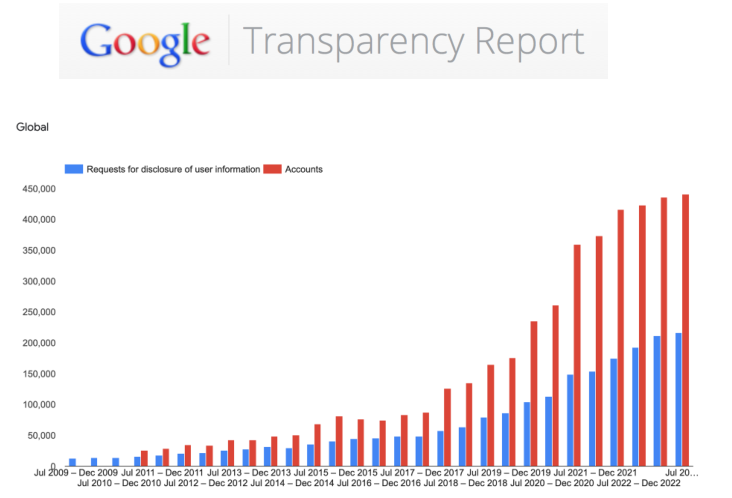
\includegraphics[width=0.6\textwidth]{img/transp_report.png}
    \caption{Timeline of Google transparency report}
    \label{fig:transparency report}
 \end{figure}

\subsubsection{Identify the suspect}
it's rigth use face recognision to identify a suspect? \\ 
For the moment if the situation is critical is possible utiliza A
live facial recognision. \\ 
AI act also regulate the use of facial recognision. % recuperare info dal testo del AI act

\subsection{Detecting and Seizing Digital Evidence}
The seize of digital evicences has torespet two foundamental rules: \textbf{bit-Stram Copy} and 
\textbf{Hash Function}. (definitions are alredy knowed)

\subsubsection{Where and how is the digital/electronic evidence hosted?}
The digital evicence can be in the suspected PC or in a third party server. \\
In the first case, we need to mange the encrition of the data, and it's possible get a Key Mandatory Law. \\
In the case of evicende in a server, is needed a collaborationfrom the ISP/Telco/Banck, and so need there is Jurisdiction problem. 

\subsubsection{The role of third paries during digital investigation}

A third party can give a lot of usefull information. \\
For example and \textbf{ISP} Could reveal from which place the email was sent, the \textbf{Mail Account Provider} could reveal from which places the email account was accessed and a \textbf{Credit Card Company} could reveal where the goods bought with a cloned credit card were delivered

\subsection{Validating Digital Evidence}
There is some tool that help to valdiate online digital evidence. \\
These kind of tool are usefull during OSINT bacasue they permit to collect data (like a story, a reel), that are not sure remain online, in a proper way for a court.


\subsection{Chain of Custody}

Digital storage media last less than analogue media and devices to read such media last even less. For example a LaserDisc last only 15 years, where there are books form thr 1086 (domesday book). So there at the moment, for trial, there are a lot of hard drive keeped in proprer way to avoid the data loss. It's a real mess.


\subsection{Analysis of Digital Evidence}

Start after the sieze of suspect's device, and need to be performed besided a precise chain of custody. \\ To perform the analysis are usually used some automatic tools, but in the recent time are used also some AI tools but only for post analysis and not for prediction policies (limitation imposed by the AI act) for example AI can not be used for kidnapping cases because the crime is in progress and not "finished".

\begin{itemize}
    \item \textbf{Text searches:} aimed at scanning files, directories and even entire file systems for specific text terms (generative AI can be used for summarizing and analyzing documents, but it's not very precise, plus alucination)
    
    \item \textbf{Image searches:} aimed at identifying image files in various formats, and at generating still frames of digitally stored video footage. Mainly analysis of child pornography that can be lead also to false positive (like a video of a mum and child in a bath)
    
    \item \textbf{Data recovery:} aimed at recovering all files stored on mass memory units, including deleted or damaged data. Destroy data can also be a crime (even if there are some backups), based on the intention of the crime (like delete file to hide evidence) 
    
    \item \textbf{Data discovery:} targeted at accessing hidden, encrypted or otherwise protected data
    
    \item \textbf{Data carving:} focused on reconstructing damaged files by retrieving portions of their content
    
    \item \textbf{Metadata recovery and identification:} this digital forensic tool is particularly useful for retracing the timeline of web accesses and file changes
\end{itemize}

Some other problem withthe use of \textbf{AI for prediction} of crime are: the bias of the AI and possible conseguences for privacy and \textbf{social control} by not very democratic government. 

\subsubsection{Two Italian issues}

\paragraph{Repeatable or Unrepeatable forensics analysis: }
\textbf{Repetable} when you can do a bit-stream copy of the data and also give one copy to the defence to do the same analysis, and more in general i can repeat analysis again and again (when i want). \\ In a \textbf{non-repetable} analysis, we need do live forensics activity and ofter occure with mobile phone, where there isn't the possibility to do a bit-stream copy of the data. In the live forensics i also need the presence of the attorney or the defender when i do the analysis to make it admissable in court.

\paragraph{Open Source or Closed Source:} %% recuperare da lezione
Open source can be more transparent 

\subsection{Presentation in Court}

The presentation of digital evidence findings is a \textbf{crucial stage} for prosecutors, judges, and lawyers (the evidence need to be presented in a way that the judge can understand it otherwire he can ignor it). The outcome of the trial relies not only on the results of the investigation but also on the \textbf{clarity and comprehensibility} of the report provided. \\

\textbf{Operational Recommendations:}
\begin{itemize}
    \item \textbf{Presence of an index:} The report should include a clear index for easy navigation through the document.
    \item \textbf{Glossary and Reference Notes:} If technical terms are used, a glossary and reference notes should be provided to ensure that all parties understand the terminology (judge and lawyers are not IT experts).
    \item \textbf{Timeline Table and Flow Charts:} A timeline table or flow charts should be included to visually represent the sequence of events and digital activities.
    \item \textbf{Presentation Slides with Photos:} Visual aids, such as presentation slides with photos, help in simplifying complex technical details.
    \item \textbf{Video Recording:} Where applicable, video recordings of the operations carried out during the investigation can provide further clarity.
\end{itemize}

\subsubsection{Presentation in Court of the Digital Evidence Findings: Murtha Case}

%% recuperare da lezione


\section{Privacy and Due Process Rights}

\subsection{Encryption}
Encryption can be used to hide the fact that encrypted messages are exchanged and used by criminals can lead to difficulties collecting the necessary evidence

\begin{figure}[!ht]
    \centering
    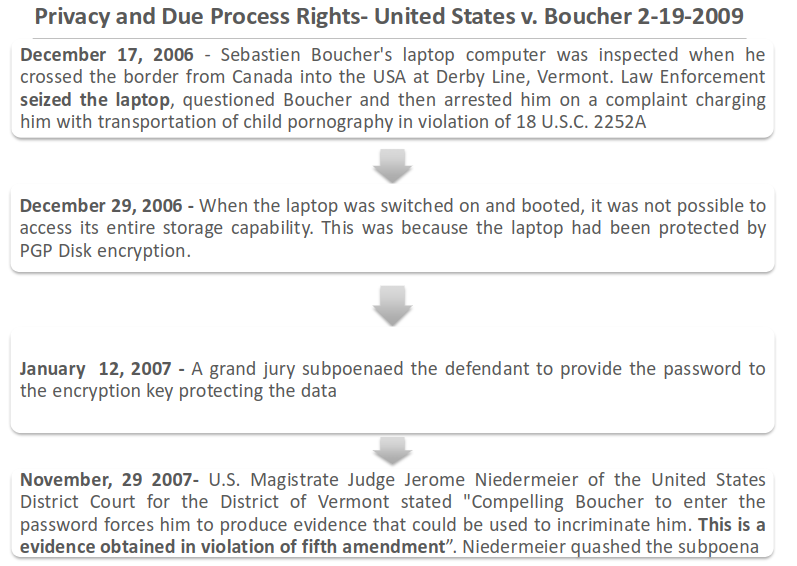
\includegraphics[width=0.5\textwidth]{img/enc_case.png}
    \caption{Case correlated with the use of encryption}
    \label{fig:encryption process}
\end{figure}

\newpage
\subsection{Case Law on Encryption}
Anther the previus case, some state are starting to create law about “Mandatory Key Disclosure" that force the suspect to give the key/password to decrypt the data. (some are Australia, Belgium France etc\dots) 

\subsection{Mandatory Key Disclosure Laws}
These case of legislative instrument doesn't work fow two main reason:
\begin{itemize}
    \item \textbf{technical reason:} An expert could always find a way yo hide a file
    \item \textbf{Possible violation of European Convention on Human Rights:} Article 6 Everyone charged with a criminal offence shall be presumed innocent until proved guilty according to law
\end{itemize} 

%% recuperare da lezione ---------

\subsection{Remote Forensics}

\begin{figure}[h!]
    \centering
    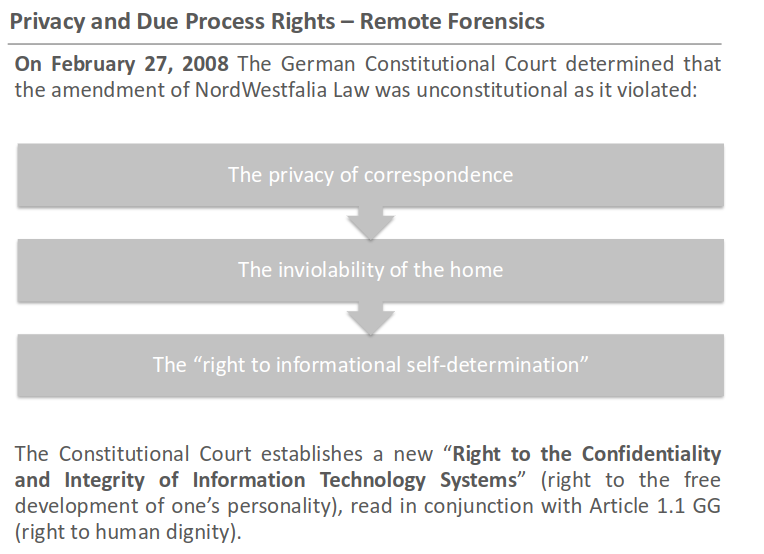
\includegraphics[width=0.4\textwidth]{img/remote_case.png}
    \caption{Case correlated to remote forensics}
    \label{fig:remote process}
\end{figure}

\subsection{Cloud Computing}

Cloud computing services face two key legal challenges: \textbf{Jurisdiction} and \textbf{Privacy}.

\paragraph{Jurisdiction}
The “\textbf{loss of location}” of digital evidence in the cloud introduces significant jurisdictional issues. In a cloud environment, the question arises: are the documents governed by the laws of the state in which they are physically located, the location of the company possessing them, or the laws of the state where the individual resides?

Over the last few years, various legal frameworks and approaches have been proposed to address this complex issue, but it remains an area of ongoing debate.

\paragraph{Privacy}
Cloud computing introduces several privacy concerns, including:
\begin{itemize}
    \item \textbf{Lack of Control:} Cloud clients may no longer maintain exclusive control over their data, limiting their ability to implement necessary technical and organizational measures to comply with \textbf{Data Protection Laws}.
    \item \textbf{Absence of Transparency:} Cloud providers may not provide sufficient information regarding how data is processed, leading to significant risks in terms of compliance with data protection regulations.
\end{itemize}


\subsubsection{Lack of control over the data} 
\begin{figure}[h!]
    \centering
    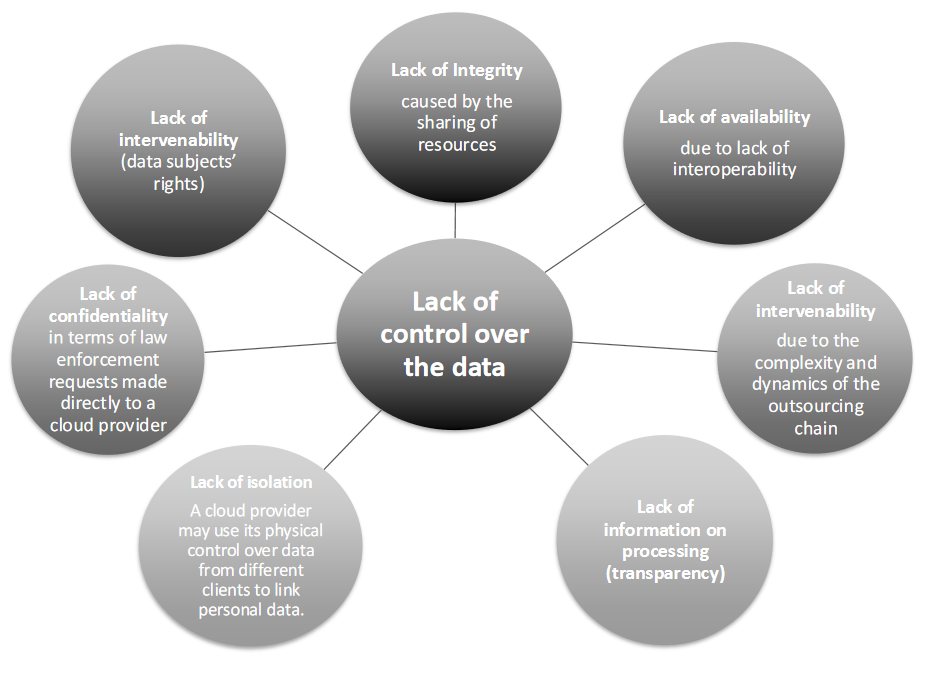
\includegraphics[width=0.5\textwidth]{img/cloud_lack_ctrl.png}
    \label{fig:lack_of_control}
\end{figure}



\subsubsection{Jurisdiction}  %% check, testo da GPT

In addressing the “loss of location” issue within the realm of cloud computing, we have four possible legal principles that can be applied:

\begin{itemize}
    \item \textbf{Territorial Principle:} The court in the jurisdiction where the data is physically located has authority. Jurisdiction is determined based on the geographical location of the data.
    
    \item \textbf{Nationality Principle:} The nationality of the perpetrator is used to establish criminal jurisdiction. The legal framework of the country of the individual committing the crime applies.
    
    \item \textbf{Flag Principle:} This principle applies to crimes committed on ships, aircraft, and spacecraft. They are subject to the jurisdiction of the country whose flag the vehicle flies under.
    
    \item \textbf{Power of Disposal Approach:} This approach focuses on who has control over the data. A regulation based on this would enable law enforcement to access a suspect's data in the cloud, regardless of its physical location, by considering the individual or entity with power over the data.
\end{itemize}

%% ------------------------------------
\chapter{Convention on Cybercrime}

\section{E-commerce on Dark Web}

\subsection{Silk Road}

\section{History and objectives of the Convention on Cybercrime (Budapest Convention)}

\subsection{Budapest Convention on Cybercrime }
%% overview direttamente nella section

\subsubsection{Timeline and Ratifications}

\subsubsection{Criticism and Opposition}


\subsection{New Global Cybercrime Treaty (UN, August 8, 2024)}

\subsubsection{Aim of the convention}

\section{Harmonization of national laws and international cooperation}


\chapter{Italian Law n. 48/2008}

\section{Overview and Significance of Italian Law n. 48/2008 in the Context of Cybercrime in Italy}

The Budapest Convention on Cybercrime was issued by the Council of Europe on November 23, 2001. Italy ratified the Convention with Law n. 48, after 7 years, on March 18 2008, which was published in the Official Gazette on April 4, 2008. But not all the principles presnet in the convention went conveted to law.


\subsection{Budapest Convention on Cybercrime - Overview}

The ratification of the Budapest Convention by Italy through Law n. 48/2008 represents a critical step in modernizing the Italian legal system to tackle cybercrime. This law aims to harmonize legal standards across borders, emphasizing the importance of international cooperation in addressing the rapidly evolving digital landscape. However, challenges remain in adapting to rapid technological changes, and continuous updates to legislative tools are necessary.

\section{Main Innovations Introduced}

\begin{itemize}[itemsep=0pt]
    \item \textbf{International harmonization of legislations:} aligning laws internationally to combat cybercrime
    \item \textbf{Reorganization of cybercrime offenses:} amendments and integrations to the penal code, introducing new specific offenses
    \item \textbf{Corporate Liability:} extending the liability under Legislative Decree 231/2001 to cover certain cybercrime offenses
\end{itemize}

\subsection{Corporate Criminal Liability}

The law extends corporate criminal liability for offenses committed in the interest or for the benefit of the company, as regulated by Legislative Decree 231/2001. This applies to all legal entities, even foreign companies if the offense is committed in Italy, for the interest or for the benefit of the company. The liability extends to offenses such as:

When the offence is committed by:
\begin{itemize}[itemsep=0pt]
    \item \textbf{Persons holding a position of representation}, management or direction or who exercise, even if de facto, management and control ("Top Management")
    \item \textbf{Persons subject to the control} or monitoring activity of the Top Management.
\end{itemize}

\begin{boxH}
    So there are 2 trials that procede in parallel, one for the company and one for the individual. And if it's proved that the action was done in the interest of the company, the company is liable.
\end{boxH}

\begin{multicols}{2}
\begin{itemize}[itemsep=0pt]
    \item Crimes against public administration
    \item Tax offenses
    \item Money laundering / receiving stolen goods
    \item Organized crime offenses
    \item Computer crimes
    \item "Corporate" offenses (including private to private corruption)
\end{itemize}
\end{multicols}

\begin{boxH}
    The company over the traditional defence could demostrate that have a compliance program in place, so a series of policies that are designed to prevent the commission of crimes, and the employee have broke them. Are often called \textbf{Soft Law}
\end{boxH}

There aren't poilices for avoid all the crimes, but if an employee commit a crime, without break the company policies, the company can can avoid the liability if the policies are recognize as valid ("the employee is too good").

\subsection{Further Innovations}

Additional measures introduced include:

\begin{itemize}
    \item Establishment of a fund under the Ministry of the Interior to combat child pornography online.
    \item Updates to data retention laws with reference to Directive 2006/24/EC.
    \item Enhancement of international cooperation, especially concerning mutual assistance in cybercrime investigations.
    \item Acquisition of digital evidence: Updates to criminal procedure code for regulating the collection and use of digital evidence.
\end{itemize}

\section{Key Provisions and Their Implications for Digital Forensics}

\subsection{Major Procedural and Investigative Updates}

\subsubsection{International Cooperation}
The law enables the Ministry of the Interior or designated authorities to instruct internet and telecommunications providers to retain and protect traffic data for up to 90 days. This period can be extended to six months for specific investigative needs, but excludes the content of communications.

\subsubsection{Competence for Investigations and Prosecutions}
Cybercrime investigations and prosecutions are assigned to the Public Prosecutor’s Office at the Court of Appeal’s main district. This aims to improve coordination in cybercrime cases. However, initial issues arose due to the lack of transitional provisions for ongoing investigations, which were later addressed by Law n. 125 of July 2008.

\subsubsection{Service Providers' Role}
Service providers, including internet, telecommunications, and postal services, play a key role in combating cybercrime. Their responsibilities include:
\begin{itemize}
    \item Retention of traffic data and communication logs.
    \item Seizure of correspondence, including electronic communications, when linked to criminal investigations.
    \item Seizure of digital data, ensuring that original data is preserved while copies are made without modification.
\end{itemize}

\subsubsection{Legal Recognition of Computer Forensics}
The law introduces computer forensics as a significant element of investigative practices, with clear protocols for handling digital evidence. These practices will need continuous updates as technology evolves.

\subsection{Best Practices in Digital Evidence Handling}
The law advocates for "best practices" in digital evidence handling, emphasizing the importance of:
\begin{itemize}
    \item Acquiring evidence without altering the original device.
    \item Authenticating both the evidence and its digital copy.
    \item Ensuring that the examination process is repeatable.
    \item Maintaining impartiality in technical analysis.
\end{itemize}

\subsection{Email Seizures}
The law also includes provisions for seizing email communications, granting the same legal protections to both traditional and electronic mail.

\subsection{Changes to the Code of Criminal Procedure}
The law modifies the Code of Criminal Procedure to extend investigative measures such as inspections and seizures to digital environments. Noteworthy amendments include:
\begin{itemize}
    \item \textbf{Digital Inspections and Searches:} Technical measures must be implemented to preserve the integrity of the original data and avoid alterations.
    \item \textbf{Preservation Orders (Freezing):} These orders are introduced as a quick measure to secure digital evidence before it can be lost or tampered with.
\end{itemize}

\section{Law n. 48/2008: Areas for Improvement}

\subsection{Standardization of Digital Evidence Procedures}
Law n. 48/2008 established a unified approach for handling digital evidence in criminal proceedings. This standardization focuses on the acquisition, preservation, and presentation of digital evidence, ensuring its integrity and authenticity for admissibility in court.

\subsection{Judicial Expertise and Training in Digital Forensics}
The implementation of this law has increased the responsibility of legal professionals to understand digital forensics. There is a growing need for specialized training in this area to avoid misinterpretation of digital evidence.

\subsection{Legal Certainty and Data Integrity}
Ensuring the integrity and authenticity of digital data is crucial. Law n. 48/2008 improved the reliability of digital evidence in court by requiring that data remain unaltered during acquisition and preservation. However, further refinement of these procedures is necessary, especially with the rise of more sophisticated cyber threats.

\section{Case Studies and Practical Applications of Italian Law n. 48/2008}

\subsection{Case Study 1: Data Seizure and Service Providers}
Phishing cases often involve the seizure of data from service providers to trace illegal transactions. Although no specific case is named, this method is frequently used in investigations of fraud and financial crimes.

\subsection{Case Study 2: Organized Crime and Communication Monitoring}
A significant case involved intercepting communications of mafia organizations in Italy. This was part of a broader initiative coordinated with Europol and Interpol, utilizing advanced digital forensic techniques to collect evidence from encrypted messages.

\subsection{Case Study 3: Cyberstalking}
In several cyberstalking cases in Italy, digital forensics were employed to trace online threats' origins. Investigators successfully identified offenders through data traffic analysis and IP identification, making this a common approach in Italian jurisprudence.

\section{Types of Corporate Investigations}
\begin{itemize}[itemsep=0pt]
    \item \textbf{Unfair Competition:} Investigating unethical practices by rival businesses.
    \item \textbf{Industrial Espionage:} Uncovering the theft of trade secrets and proprietary information.
    \item \textbf{Employee Misconduct:} Addressing violations of company policies and contracts.
    \item \textbf{Intellectual Property Infringement:} Protecting copyrights, trademarks, and patents from unauthorized use.
\end{itemize}

\section{Man-in-the-Middle (MITM) Attacks}
MITM attacks represent a silent and sophisticated form of cybercrime where an attacker intercepts communication between two parties. This allows criminals to monitor, read, and modify messages undetected, often targeting businesses involved in international trade. \bigskip

The attack's success relies on the attacker's ability to remain undetected while gathering crucial information \textbf{over an extended period}.

\subsection{The Mechanics of MITM Attacks}
\begin{itemize}[itemsep=0pt]
    \item \textbf{Initial Breach:} Hackers compromise a company's email system through methods such as phishing, brute force attacks, or trojans.
    \item \textbf{Monitoring Phase:} Attackers observe communications over time, gathering information on business practices and relationships.
    \item \textbf{Interception:} At an opportune moment, criminals intercept and alter payment instructions, redirecting funds to their accounts. When one party requests a payment, the attacker sends fraudulent account details to the other party (like by editing the mail with the invoice).
    \item \textbf{Execution:} Unaware of the fraud, victims transfer funds to the fraudulent account, often resulting in significant financial loss.
\end{itemize}

\subsection{Legal Implications of MITM Attacks}
\textbf{Criminal Perspective:} MITM attacks can be classified as fraud under Article 640 of the Italian Criminal Code, involving deception through false emails and documents. \textbf{Identity Theft:} Such attacks may also fall under identity substitution (Article 494) and computer fraud (Article 640 ter), particularly with recent legislative changes.

\subsubsection{Jurisdictional Challenges}
Prosecution of MITM attacks is often complicated by jurisdictional issues and time constraints, as attackers frequently operate from countries with limited judicial cooperation.

\subsection{Civil Recourse and Bank Responsibilities}
\textbf{Immediate Action:} Victims should promptly request payment reversals while funds remain in the destination account. Some European banks may assist by freezing accounts and returning funds.

\textbf{Bank Liability:} European regulations, such as the Payment Service Regulation and Italian Legislative Decree 27 January 2010, n. 11, often shield banks from liability, even when account holder details do not match.

\textbf{Regulatory Gaps:} Current regulations may be insufficient in an era of fast online payments, where financial intermediaries predominantly control transaction verification.

\chapter{UN Resolution on Cybercrime}

\section{Background and Objectives of the Resolution}
The primary objective of this resolution is to initiate the drafting of a global treaty aimed at combating cybercrime through multilateral negotiations. The title, "Countering the use of information and communications technologies for criminal purposes," signifies a step towards developing an international convention on cybercrime, targeting the implementation of concrete measures against this form of crime. \bigskip

The resolution establishes a dedicated Committee responsible for drafting a comprehensive convention. This process is expected to be transparent, involving a wide range of stakeholders, such as developing countries, intergovernmental organizations, and field experts.

\section{Impact on International Cybersecurity Policies and Practices}

\subsection{UN Resolution (26 May 2021)}
This resolution could significantly impact international cybersecurity policies, promoting greater cooperation and harmonization among states. By establishing shared minimum standards through an international cybercrime treaty, it fosters a more unified regulatory framework and enhances investigative cooperation across different jurisdictions. \bigskip

The adoption of the resolution required various amendments and compromises, highlighting the importance of balancing national and supranational interests while ensuring inclusivity and transparency.

\subsection{Human Rights and Privacy Risks}
One of the central issues discussed in the UN report is the need to balance cybersecurity measures with the protection of human rights, particularly privacy and data protection. Although there is a consensus on the importance of cybersecurity, the UN GGE report warns against overreach, as unregulated measures may infringe on civil liberties.

\subsection{Emerging Threats and Supply Chain Integrity}
The report emphasizes the growing risks associated with vulnerabilities in global supply chains, especially in the ICT sector. Such vulnerabilities could lead to large-scale attacks or espionage, underlining the need for states to secure digital infrastructures and collaborate on emerging threat information.

\section{Future Legal Framework for Cybersecurity}
Cybersecurity policymakers are required to implement stringent measures to protect data during investigations. Legislative provisions should allow for periodic review and updates to cybersecurity practices, ensuring adaptability to evolving digital threats.

\section{Analysis of Key Components and Legal Implications of the
Resolution}

\subsection{Ad Hoc Committee}
The resolution establishes an Ad Hoc Committee to draft a global cybercrime convention. This committee is mandated to convene at least six times, each session lasting 10 days, beginning in January 2022. Decisions within the committee are expected to be made by consensus or, failing that, by a two-thirds majority.

\subsection{Cyber Sovereignty and Legal Boundaries}
The concept of cyber sovereignty presents a significant legal challenge. Countries such as China and Russia advocate for state control over cyberspace, potentially clashing with international norms of internet freedom and openness. The UN resolution seeks to address these tensions, but the broader debate over the degree of state control in cyberspace governance remains unresolved, necessitating a balance between sovereignty and global cooperation.

\subsection{Public-Private Cooperation and Liability}
Legal frameworks must account for the increasing role of private companies in cybersecurity. The resolution encourages collaboration between states and private entities, such as internet service providers and cybersecurity firms, to counter cyber threats. This approach raises legal questions concerning the responsibility and liability of these companies, especially when they participate in responding to or preventing cyberattacks.

\section{Jurisdictional Provisions (Article 22)}

\subsection{Territorial Jurisdiction}
State Parties must establish jurisdiction over offenses committed within their territory or on vessels or aircraft registered under their laws.

\subsection{Extended Jurisdiction}
States may also establish jurisdiction over offenses that:
\begin{itemize}
  \item Are committed against their nationals.
  \item Are committed by their nationals or stateless persons
    habitually residing within their territory.
  \item Are committed outside their territory with the intent of
    carrying out an offense within their territory, as specified in
    Article 17 of the Convention.
  \item Are committed against the State itself.
\end{itemize}

\subsection{Jurisdiction and Non-Extradition}
If the alleged offender is present within a State's territory and not extradited solely due to nationality, the State must establish jurisdiction over the offense. In cases where extradition is denied for other reasons, States may take additional measures to establish jurisdiction.

\subsection{Coordination Among States}
When a State exercising jurisdiction becomes aware of other States conducting investigations or proceedings for the same offense, authorities are encouraged to consult and coordinate their actions.

\subsection{Compatibility with International Law}
This Article affirms that the Convention does not prevent any State Party from exercising other forms of criminal jurisdiction, as permitted by its domestic law.



\section{Garlasco Case}
Digital evidence could be altered and can contain countless pieces of information. The “Garlasco” case is a clear example of this. \bigskip

Alberto Stasi was acquitted of the murder of his girlfriend, Chiara Poggi, by the Court of First Instance in December 2009, and the judgment was confirmed in the Appeal court in December 2011.

\section{Italian Case Law on Digital Forensics}
\begin{itemize}
    \item \textbf{13/08/07:} Stasi wakes up at 9, telephones Chiara Poggi, works on his thesis.
    \item \textbf{14/08/07:} Chiara Poggi died between 10:30 and 12:00.
    \item \textbf{29/08/07:} Stasi voluntarily hands over his PC to the Police.
    \item \textbf{17/12/09:} Judge Vitelli acquits Stasi of murder.
\end{itemize}
The expert report requested by the judge shows that Stasi was working on his thesis during the period when Chiara Poggi was killed.

\section{The Internet of the Human Body: Towards a Habeas Data?}
\begin{multicols}{2}
    \begin{quote}
        “If your internet thermostat's pinging servers all day, will the cops think you're a weed farm? Or just a hot yoga gym?" \\ \textit{Jonathan Zittrain}
    \end{quote}

    \begin{quote}
        “Sure, encrypt your email – while your shiny IoT toothbrush spies on you” \\ \textit{Susan Landau}
    \end{quote}
\end{multicols}

\newpage

\section{Cases}

\subsection{Connie Debate Case: Fitbit}

\begin{multicols}{2}
    \begin{quote}
        “As people continue to provide more and more personal information through technology, they have to understand we are obligated to find the best evidence, and this technology has become a part of that.”  \\
        \textit{Detective Christopher Jones - East Lampeter Township Police Department in Pennsylvania}
    \end{quote}

    \begin{quote}
        “We are entering an era of sensorveillance. People are just waking up to the fact that their smart devices are going to snitch on them and that they are going to reveal intimate details about their lives they did not intend law enforcement to have”  \\
        \textit{Andrew Ferguson, a University of the District of Columbia law professor}
    \end{quote}
\end{multicols}



\subsection{James Bate Case: Amazon Echo}

\begin{multicols}{2}
    \begin{quote}
        “The Amazon Echo device is constantly listening for the 'wake' command of 'Alexa' or 'Amazon,' and records any command, inquiry, or verbal gesture given after that point”  \\
        \textit{Search Warrant}
    \end{quote}

    \begin{quote}
        “The allegation that the Echo is possibly recording at all times without the wake word being issued is incorrect”  \\
        \textit{Answer of an Amazon Representative}
    \end{quote}
\end{multicols}

There are prloblems with the term and conditions of the Amazon Echo, as they are record data even without the wake word being issued. This is also correlated with all the problem reguardind the user of dark pattern for avoid that the use could block this kind of data collection. \\
In another case Amazon refused to give data collected by an Amazon echo to the police and use the term and conditions as exuse. \bigskip

NOTE: particularly attection for device that arrive from China (alsways check the user term and conditions).

\subsection{Ross Compton Case: Pacemaker}

\begin{multicols}{2}
    \begin{quote}
        “There is a lot of other information about things that may characterize the inside of my body that I would much prefer to keep private rather than how my heart is beating. It is just not that big of a deal” \\ 
        \textit{Judge Charles Pater}
    \end{quote}

    \begin{quote}
        “Americans shouldn't have to make a choice between health and privacy. Compelling citizens to turn over protected health data to law enforcement erodes those rights.”  \\
        \textit{Electronic Frontier Foundation Attorney Stephanie Lacambra}
    \end{quote}
\end{multicols}

Accused of frode from the incusance (hose burn), at the end of the process, the judge accept to aquire the data from the peace maker, to check the beat of the heart at the time of the incident. \bigskip

Inside our body there are a lot of data that could be used for the investigation, but the question is: how much of this data could be used for the investigation? 

\section{Facial Recognition Biometric Border}

\begin{multicols}{2}
    \begin{quote}
        “U.S. Customs and Border Protection says it will delete the live photos captured at the gate within 14 days for citizens, and that it only uses them to verify identity by comparing them with the database photos”  \\
        \textit{CBP Privacy Impact Assessment}
    \end{quote}

    \begin{quote}
        “Face Recognition has a great potential for expansion and misuse: for example, you can subject thousands of people to face recognition when they’re walking down the sidewalk without their knowledge”  \\
        \textit{Senior Policy Analyst, ACLU - Jay Stanley}
    \end{quote}
\end{multicols}

In europe there is a law that proibit the use of facial recognition in real time for the identification of the people, but in the US this is not the case. \bigskip

\section{Categories of Law Enforcement Activity}

\begin{itemize}[itemsep=0pt]
    \item Situations involving officers observing an ongoing crime (\textbf{FaceFirst})
    \item Situations involving officers investigating a past crime \textbf{(KeyCrime$^3$)}
    \item Situations involving officers predicting a future crime (\textbf{PredPol}, used in US, illegal in EU for AI act) \\ Tool for analysze crime that could happen in the future baed on the use of bigdata from the db of the law enforcement and social media data. \\ The problem for the critisim is that if you predict a crime in a certain area, the police will go in that area and this could lead to a self-fulfilling prophecy.
\end{itemize}

\section{“Police” Directive}

The Pocile Directive can be seen as a GDPR for the police. It is composed by 5 pillars:

\begin{itemize}[itemsep=0pt]
    \item Fairly, lawful, and adequate data processing during criminal investigations or to prevent a crime
    \item Clear distinction of various categories of data subjects in a criminal proceeding (investigated person, person convicted, victim of crime, third parties to the criminal offense)
    \item Prohibit measures that produce adverse legal effects for the data subject based solely on automated processing of personal data
    \item Implementation of privacy by design and by default mechanisms to ensure protection of data subject rights and minimal processing
    \item Cooperation with relevant supervisory authorities, providing all necessary information for their duties
\end{itemize}

\section{Automated Processing (Article 11 - “Police Directive”)}

Automated processing is forbidden unless:
\begin{itemize}[itemsep=0pt]
    \item \textbf{Human Intervention:} Automated processing is forbidden unless:
    \begin{enumerate}[itemsep=0pt,  label=\roman*.]
        \item There is human intervention
        \item Produce an adverse legal effect concerning the data subject
        \item Is authorized by UE or Member states
        \item Provides appropriate safeguards for the rights and freedoms of the data subject
    \end{enumerate}
    \item \textbf{Profiling:} Profiling that results in discrimination against natural persons on the basis of special categories of personal data referred to in Article 10 shall be prohibited, in accordance with Union law.
    
    \item \textbf{Access to electronic:} Legislation permitting public authorities to gain access to the contents of electronic communications on a generalised basis must be regarded as compromising the essence of the fundamental right to respect for one’s private life, as guaranteed by Article 7 of the Charter
\end{itemize}

\section{Transparency, Retention, and Enforcement}

\begin{itemize}[itemsep=0pt]
    \item \textbf{Transparency}: Tools based on big data for law enforcement purposes is checked by the law enforcement authority prior to final purchase and can be verified for its suitability, correctness and security, bearing in mind that transparency and accountability are limited by proprietary software
    \item \textbf{Retention}: While EU legal framework on data retention still lacking and we are waiting the Guidelines, safeguards are required for data retention to be lawful according to the ECJ case law are: 
    \begin{enumerate}[itemsep=0pt, label=\roman*.]
        \item serious crime;
        \item necessary and proportionate retention measure;
        \item national authorities’ access should meet certain data protection safeguards
    \end{enumerate}
    
    \item \textbf{Enforcement}: Member States shall lay down the rules on penalties applicable to infringements of the provisions adopted pursuant to this Directive and shall take all measures necessary to ensure that they are implemented. The penalties provided for shall be effective, proportionate and dissuasive
\end{itemize}

\section{Privacy vs Security}

\textit{What happens if security prevails over privacy?} - Netflix case

\section{Budapest Convention on Cybercrime - Overview}

The Budapest Convention on Cybercrime was issued by the Council of Europe on November 23, 2001.  
Italy ratified the Convention with Law n. 48 on March 18, 2008, and it was published in the Official Gazette on April 4, 2008.
\chapter{Hacking Team Case Study}
\section{Hacking Team Case}

\section{Background on Hacking Team}
Hacking Team was an Italian technology company primarily known for its offensive intrusion and surveillance software provided to government bodies and law enforcement agencies across the globe. Established in 2003, the company garnered significant controversy due to its practices and clientele, which included both national security organizations and regimes with questionable human rights records.

\subsection{Company Overview}
\begin{itemize}
    \item \textbf{Founded:} The company was established in Milan, Italy, by David Vincenzetti in 2003.
    \item \textbf{Business Model:} Hacking Team specialized in creating and selling offensive cybersecurity tools tailored for governmental and law enforcement agencies, focusing on hacking and surveillance applications.
    \item \textbf{Key Clients:} The client list reportedly included major international organizations such as the NSA, CIA, FBI, and other international law enforcement agencies.
\end{itemize}

\section{Core Technologies}
Hacking Team developed advanced tools to enhance surveillance capabilities for their clients, often pushing the boundaries of intrusion technology.
\subsection{Remote Control System}
A software solution enabling monitoring of Internet communications, data decryption, and activity tracking.
\subsection{Mobile Surveillance}
Technologies designed for tracking cell phones, monitoring calls, and intercepting messages.
\subsection{Remote Activation}
Tools capable of remotely activating microphones and cameras on target devices, including precise location tracking.
\subsection{Advanced Surveillance Techniques}
\begin{itemize}
    \item \textbf{Battery Optimization:} Techniques to minimize battery usage on monitored devices, reducing suspicion from the target.
    \item \textbf{Stealth Operations:} Surveillance procedures developed to be highly undetectable.
    \item \textbf{Data Extraction:} Sophisticated methods to extract and analyze data from target devices effectively.
\end{itemize}

\section{Founding and Early Years}
\begin{itemize}
    \item \textbf{2003:} David Vincenzetti and Valeriano Bedeschi founded the company in Milan.
    \item \textbf{2007:} Hacking Team received \$8 million in funding from Italian venture capital, supporting rapid growth.
    \item \textbf{Early Success:} The Milan police purchased Hacking Team’s software, marking it as one of the first providers of commercial hacking solutions.
\end{itemize}

\section{Applications of Technology}
Hacking Team’s technology was applied in various high-stakes operations by law enforcement agencies around the world.
\begin{itemize}
    \item \textbf{Counter-Terrorism:} Utilized to monitor and track terrorist activities, assisting in prevention and response.
    \item \textbf{Drug Trafficking:} Employed in combating international narcotics trade by tracking and intercepting key individuals and communications.
    \item \textbf{Organized Crime:} Used to gather intelligence on mafia and other criminal organizations.
\end{itemize}

\section{High-Level Connections}
\begin{itemize}
    \item \textbf{Booz Allen Hamilton:} Established connections with Mike McConnell, a former NSA director and influential intelligence advisor.
    \item \textbf{US Intelligence:} Collaborated with the NSA, CIA, and FBI, highlighting its close ties with American intelligence.
    \item \textbf{Global Reach:} Extended operations to intelligence agencies worldwide, solidifying its position in international cybersecurity markets.
\end{itemize}

\section{Saudi Arabia Acquisition Attempt}
\begin{itemize}
    \item \textbf{2013:} Initiated acquisition discussions with the Saudi Arabian government.
    \item \textbf{Valuation:} The company was valued at \$2 billion, though Saudi Arabia’s offer was approximately \$140 million.
    \item \textbf{Mediators:} Wafic Said, Britain’s third wealthiest Arab billionaire, was involved as a mediator in negotiations.
\end{itemize}

\section{Controversial Clients}
Hacking Team faced criticism for dealing with governments known for human rights abuses.
\begin{itemize}
    \item \textbf{Sudan:} Software was sold to Sudan, despite an arms embargo imposed by the United Nations.
    \item \textbf{Bahrain:} Provided surveillance technology to the Bahraini government.
    \item \textbf{Saudi Arabia:} Supplied spyware to Saudi Arabian authorities, sparking international concerns.
\end{itemize}

\section{UN Investigation}
\begin{itemize}
    \item \textbf{June 2014:} The United Nations commission raised concerns about Hacking Team’s sales to Sudan.
    \item \textbf{January 2015:} Hacking Team denied any ongoing sales to Sudan.
    \item \textbf{March 2015:} The UN suggested that Hacking Team’s software could be classified as military-grade equipment.
\end{itemize}

\section{Italian Export Ban}
\begin{itemize}
    \item \textbf{Autumn 2014:} The Italian government temporarily suspended Hacking Team’s export license.
    \item \textbf{Lobbying Efforts:} Hacking Team engaged in lobbying to reverse the export restrictions.
    \item \textbf{Ban Lifted:} The company ultimately regained the right to sell its products internationally.
\end{itemize}

\section{Ethical Concerns}
Critics raised ethical issues regarding Hacking Team’s operations and clientele.
\begin{itemize}
    \item \textbf{Human Rights:} Accused of enabling surveillance in regions with poor human rights protections.
    \item \textbf{Privacy Violations:} Tools were often used to infringe on citizens’ privacy rights.
    \item \textbf{Democratic Concerns:} Allegations of contributing to the suppression of democratic freedoms in certain nations.
\end{itemize}

\section{Legal Challenges}
\begin{itemize}
    \item \textbf{UN Sanctions:} Faced scrutiny regarding potential violations of the UN arms embargo.
    \item \textbf{Italian Export Laws:} Temporary suspension of exports by the Italian government.
    \item \textbf{Privacy Lawsuits:} Involved in legal actions in various countries related to privacy violations.
\end{itemize}

\section{The Investigation}

\section{2015 Data Breach}
In 2015, Hacking Team, ironically known for its surveillance and cybersecurity tools, became a victim of a significant cyber attack. This event had far-reaching consequences for the company and its clients.
\subsection{Event}
Hacking Team's internal systems were breached, leading to the unauthorized access and exposure of confidential information.
\subsection{Consequence}
Approximately 400 gigabytes of sensitive data were leaked, including emails, financial documents, and client communications.
\subsection{Aftermath}
The breach publicly revealed the company's internal operations, client lists, and previously confidential dealings, casting a negative spotlight on Hacking Team’s business practices and clientele.

\section{Client List and Revenue}
Hacking Team's client base and revenue streams were broad, involving high-profile organizations and substantial financial engagements.
\subsection{Client Types}
Primarily served military, police, governmental, and intelligence agencies worldwide, providing them with hacking and surveillance tools.
\subsection{Corporate Clients}
The company maintained partnerships with multinational corporations, including Boeing, expanding its influence beyond public sector organizations.
\subsection{Revenue}
Hacking Team reported annual revenues exceeding €40 million, though some reports suggested additional income from larger, undisclosed offshore contracts.

\section{Milan Prosecutor's Investigation}
Suspicious financial transactions led to an official investigation by Milan’s prosecutor’s office, which scrutinized dealings between Hacking Team affiliates and external entities.
\subsection{Trigger}
A suspicious payment from a Saudi Arabian company to SoftHack Srl, a Turin-based firm, prompted Milan prosecutor Alessandro Gobbis to order a search of SoftHack Srl.
\subsection{Action}
The prosecutor launched an investigation, focusing on possible unauthorized sales or misuse of Hacking Team's spyware technology.
\subsection{Suspicion}
It was suspected that the Galileo spyware source code may have been illicitly sold to unauthorized parties, raising concerns about its potential misuse.

\section{SoftHack Srl Investigation}
SoftHack Srl, the company at the center of the suspicious transaction, became the subject of legal scrutiny.
\subsection{Company Details}
SoftHack Srl, based in Turin, is a technology company involved in software development.
\subsection{Individual Involved}
Luca Spector, a developer associated with SoftHack Srl, was investigated under charges of unauthorized system access and disclosure of industrial secrets.

\section{Suspicious Transaction Details}
Details of the payment that triggered the investigation are as follows:
\begin{itemize}
    \item \textbf{Date:} November 20, 2014
    \item \textbf{Amount:} 300,000 euros
    \item \textbf{Sender:} Saudi Technology Development Inv.
    \item \textbf{Recipient:} SoftHack Srl
\end{itemize}

\section{Prosecutor's Suspicions}
The Milan prosecutor’s office raised concerns regarding the nature and intent of the transaction.
\subsection{Cover Story}
The payment was reportedly for “professional training services”; however, this explanation was met with skepticism.
\subsection{Real Purpose}
Investigators suspected that the true intent of the transaction was the sale of the Galileo spyware source code.
\subsection{Potential Misuse}
There were concerns that the software could potentially fall into the hands of terrorist groups or be misused for malicious purposes.

\section{Saudi Technology Development Inv}
The investigation further examined Saudi Technology Development Inv., the company involved in the suspicious payment.
\subsection{Investigation Focus}
The probe focused on the shareholders of the company and any potential connections to jihadist networks.
\subsection{Intermediary Role}
Saudi Technology Development Inv. was suspected of acting as a mediator for an unidentified client, raising questions about the true end-users of the spyware.
\subsection{Unknown Motives}
The motivations behind the acquisition of Hacking Team's software by this entity remain unclear.

\section{SoftHack's Defense}
SoftHack Srl and its legal representation denied any wrongdoing and provided clarifications regarding the transaction.
\subsection{Denial}
SoftHack’s lawyer refuted the accusations, claiming they were baseless rumors propagated by Hacking Team.
\subsection{Clarification}
The defense pointed out that the search warrant did not explicitly mention any sale of services to Arab or terrorist organizations.
\subsection{Transparency}
SoftHack expressed a willingness to cooperate fully with the investigation to demonstrate its innocence.

\section{Ongoing Investigation}
The investigation continues as authorities delve deeper into the background and potential connections of Saudi Technology Development Inv.
\subsection{Current Focus}
Efforts are centered around investigating Saudi Technology Development Inv.’s history and any links it might have to extremist groups.
\subsection{Key Question}
A primary focus of the inquiry is determining whether the spyware ultimately reached terrorist organizations or other unauthorized users.
\subsection{Next Steps}
The investigation will proceed with additional interrogations and analysis of financial transactions to ascertain the true nature of the dealings.

\section{Search and Seizure}

\section{Subject: Search and Seizure of Electronic Devices}
\subsection{Issuing Authority}
The Italian Cybercrime Unit issued a search and seizure warrant directed at SoftHack Srl's headquarters in Turin. This warrant was part of a broader investigation initiated by the Prosecutor’s Office of Milan.

\subsection{Location to be Searched}
The search specifically targets the main offices of SoftHack Srl in Turin.

\subsection{Items to be Seized}
The warrant details several categories of electronic devices that are believed to contain critical evidence for the ongoing investigation:
\begin{itemize}
    \item Laptop computers
    \item Smartphones
    \item CCTV cameras
    \item Tablets (including iPads)
    \item Other electronic devices capable of storing digital evidence relevant to the case
\end{itemize}

\subsection{Purpose of Warrant}
The warrant is part of an investigation into unauthorized access to proprietary source code owned by Hacking Team, a Milan-based intelligence software company. Evidence suggested that SoftHack Srl may have received substantial payments from Saudi Technology Development Inv., which were allegedly labeled as payments for professional training but are suspected to be in exchange for sensitive source code and proprietary information.

\section{Justification for Immediate Seizure}
The presence of specified electronic devices at SoftHack Srl is believed to hold critical evidence essential to the investigation. Immediate seizure was authorized to prevent any tampering, destruction, or concealment of data. Preserving digital evidence in its original state is necessary to maintain evidential integrity in accordance with digital forensic protocols.

\section{Digital Forensics Standards}
The execution of the warrant adheres to strict digital forensic principles to ensure evidence integrity and admissibility in court:
\subsection{Integrity of Evidence}
All electronic devices must be handled carefully to prevent any data alteration. Forensic experts are tasked with securing the devices in a controlled environment, using write-blocking tools and creating forensic images of all data prior to any detailed examination.
\subsection{Documentation and Chain of Custody}
A comprehensive log of each device seized must be maintained, detailing serial numbers, device types, and any identifiable markings. The chain of custody is recorded from the moment of seizure to the forensic examination, ensuring full transparency and traceability.
\subsection{Impartiality and Accuracy}
Digital forensics standards are strictly enforced to prevent contamination or bias. Write-protection technology and forensic imaging are essential to preserving original evidence without alteration.

\section{Execution of the Warrant}
The warrant authorizes the Italian Cybercrime Unit to enter and search the premises of SoftHack Srl, with specific attention to the electronic devices listed above. The search is to be conducted within a specified timeframe, after which all seized devices will be transferred securely to a designated forensic lab or another appropriate authority for analysis.

\section{Additional Provisions}
\begin{itemize}
    \item The warrant restricts access solely to data relevant to the investigation, and private data unrelated to the case must remain protected.
    \item All procedures are to comply with applicable data protection laws, thereby respecting the privacy of individuals not associated with the investigation.
\end{itemize}

\section{Order}
The Prosecutor’s Office of Milan issues this search and seizure warrant to be executed in accordance with the outlined digital forensic standards. The order emphasizes the importance of maintaining forensic reliability and preserving all digital evidence collected during the search.

\section{Guidelines for Prosecutor and Law Enforcement Officers}
To ensure compliance with digital forensic principles throughout the investigation, prosecutors and law enforcement officials should adhere to the following:
\begin{itemize}
    \item Respect the chain of custody and document all procedures accurately.
    \item Utilize forensic imaging and write-blocking tools to safeguard the original state of electronic evidence.
    \item Ensure the impartial handling of evidence to avoid introducing bias.
\end{itemize}

\section{Defense Strategy and Attorney’s Role}
\subsection{Attorney’s Responsibilities}
The defense attorney has a critical role in protecting the defendant's rights during the investigation:
\begin{itemize}
    \item Ensure that forensic protocols are followed, and that evidence was collected and handled legally.
    \item Advocate for the preservation of the defendant’s rights, particularly regarding privacy and protection from unlawful search and seizure.
\end{itemize}

\subsection{Demonstrating Client Innocence}
To demonstrate the innocence of the defendant, the attorney should:
\begin{itemize}
    \item Scrutinize the validity of the evidence, ensuring it was obtained without bias or procedural errors.
    \item Gather any exculpatory evidence or alternative explanations that might counter the prosecution’s allegations.
    \item Present compelling evidence to the judge, providing context to support the client's lack of involvement in the alleged wrongdoing.
\end{itemize}


\part{Tech}
\chapter{Introduction}

\section{Topics}
\begin{itemize}
  \item \textbf{Forensics Analysis} \\
    use of logic and meaningful knowledge and methodological approach to
    legal problems and criminal investigation.
  \item \textbf{Computer Forensics} \\
    Collection, preservation and analysis of digital evidence
    (inside file system, email, cloud account etc...) to support
    investigation and legal proceedings
\end{itemize}

\section{Forensics History}

\subsection{Ancient Times}
Forensic science dates back to \textbf{Babylon (1900 BC)} where fingerprints
were used for identification, and \textbf{China (1248 AC)} with forensic pathology.
In the \textbf{UK (1835)}, bullet comparison solved a case, and by \textbf{1892},
the first murder was solved using fingerprints.

\subsection{Modern Times}
Forensic standards grew in police departments, with the first crime lab in
\textbf{1923}. DNA fingerprinting began in the \textbf{1950s}, and DNA profiling
was developed by \textbf{1985}. \textbf{AFIS} systems emerged in the late
\textbf{1980s}. Today, AI, toxicology, and digital forensics are key areas
of innovation.

\subsection{Digital Field}

\subsubsection{Early Times}
In \textbf{1989}, Robert Morris was convicted under the Computer Fraud and
Abuse Act, marking the first use of computer logs in forensics. That year,
\textbf{IACIS} was founded, followed by \textbf{IOCE} in \textbf{1995} to
share digital forensic practices.

\subsubsection{Recent Times}
\begin{itemize}
  \item \textbf{1990}: Forensic tools like EnCase emerged
  \item \textbf{2000}: Digital forensics became widespread in law enforcement
  \item \textbf{2010}: Growth of cloud and mobile forensics, automation, and
    machine learning
  \item \textbf{2020}: Advances in crypto, blockchain, and AI improve digital
    forensics
\end{itemize}

\section{Computer Forensics Definitions}

\textbf{US\_CERT:} The discipline that combines elements of law and computer
science to collect and analyze data from computer systems,
networks, wireless communications, and storage devices in a
way that is admissible as evidence in a court of law. \\
\textbf{A. Ghirardini -Computer Forensics:} The discipline whose goal is preservation, identification, analysis of
information system to the aim of identification of evidences during
investigation activities. \\
\textbf{NIST glossary:} The application of computer science and investigative procedures
involving the examination of digital evidence - following proper search
authority, chain of custody, validation with mathematics, use of validated
tools, repeatability, reporting, and possibly expert testimony.

\section{CF purpose(s)}

\subsection{CF Q\&A}
During an investigation, digital forensics need to analysis data to answer some key questions: \\
\begin{minipage}[t]{0.45\textwidth}
  \begin{itemize}
    \item \textbf{What happened?}
    \item \textbf{Who was involved?}
    \item \textbf{When did it take place?}
  \end{itemize}
\end{minipage}
\begin{minipage}[t]{0.45\textwidth}
  \begin{itemize}
    \item \textbf{Where did it take place?}
    \item \textbf{Why did it take place?}
    \item \textbf{How did an incident occur?} \newline
  \end{itemize}
\end{minipage}

The answers to these questions are essential for support legal proceedings and mitigate
possibility of future incidents with a preventive approach.

\subsection{CF Goals}

The goals of computer forensics (CF) are multifaceted and aim to provide a
comprehensive understanding of digital incidents. \\
Firstly, CF seeks to retrieve what has been the input, such as what has been typed.
It also aims to determine the actions performed, for example, what programs have been run
and what peripherals have been connected. \\
Additionally, CF involves analyzing used files to understand what modifications
have been done and when these modifications occurred (and the information from an OS
  are not enougth, because are an abstraction managed by the file system $\rightarrow$ needed
bit analysis (like for ereased data)). \\
Another critical goal is to identify the damage done,
such as what data have been erased. In essence, the overarching goal
of CF is to \textbf{gain a technical comprehension of what happened during the
incident} (from a technical point of view).

\chapter{CF Terminology \& revelant conceps}

\section{Terms}

\subsection{Digital evidence}
Technical definition of Digital evidence is very similar to the legal ones:
\begin{boxH}
  Data stored or transmitted in digital form that can be used in court.
\end{boxH}

The conrnerstones of digital forensics are the different levels of \textbf{abstraction}, requires
\textbf{interpretation}, are \textbf{fragile}, may be \textbf{voluminous}
and the difficulty to discover \textbf{connection} between
data and reality (the connection need to be done beafore entering the court). \\

Digital evidence also requires a deep technical understanding of the possible types of data
(files, emails, logs, metadata) and the legal requiremnets for each of one to collect and preserve it.
(To make all of this effective, knowledge of file systems, network protocols
and encryption are essential) \\

\subsection{Chain of custody}
\begin{boxH}
  Documented and \textbf{unbroken} process of handling evidence
  from the time it is collected until it is presented in court
\end{boxH}

This procedure is essential to ensure the integrity of the evidence and to avoid
that them to be tampered or accessed by unauthorized people. \\
Keep the chain of custody requires knowledge about how to document evidence
collection, storage, and access (logging procedures, secure storage, legal prtocols etc..) \\

If the chain of custody is \textbf{broken}, the evidence may be considered \textbf{inadmissible in court}
(so is needed know the regulation of the state to decide how to manage it).

\subsection{Data acuisition}
\begin{boxH}
  The process of collecting digital evidence from devices
  without altering or damaging the original data.
\end{boxH}

One of the biggest problem fo the managment of digital evidence, because it's needed to be performed
on hostile systems (that can be infected, compromised, have a malware or system to avoid copy
like edited system call for make other program to fail). in a not coltrolled envorment like a crime scene. \\
So are needed knowledge of disk imaging and live data capture in order to not alter what's going on
on the suspect system. Are also required expertise in forensics acquisition, analysis
tools (like FTK Imager, EnCase) and knowledge of file systems, write-blockers, and hashing
(crucial for ensuring integrity).

\subsection{Hashing}
\begin{boxH}
  The process of converting data into a fixed-length string of
  bits, which represents the data uniquely
\end{boxH}

It's used in the chain of custody for ensure the integrity of the digital evidence and so verity
that a file has not been altered. \\
Require understanding of hashing algorithms (strengths and
weaknesses, e.g. MD5 collision), formats
(hex, base64 etc...) (if wrong formats are sued, the chain of custody is broken and each information
gathered from that point is considered not valid)
and expertise in hashing tools (sha256sum, hashdeep, FTK imager, Autopsy). \\

Have to be used any time an evidence is "managed" (copied, moved)

\subsection{Write Blocker}
\begin{boxH}
  Hardware or software tool used to prevent any data from
  being written to a storage device during analysis, preserving
  the original data content
\end{boxH}

To be operated, require understanding of how write-blocking devices work
and how they can be implemented in forensic procedures. \\

It's essential for the legally defensible acquisition.

\subsection{Forensic image}

\begin{boxH}
  A bit-by-bit copy of digital media, including deleted files and
  data in slack space, which is an exact replica of the original device
\end{boxH}

The goal of a forensic image is to preserve the original evidence and aovid the modification
of the original data. \\

To be performed in a correct way, requires understanding of mechanisms to copy information
in digital devices (file system knowledge and behavior) and familiarity with  with bit-by-bit copy tools
(DD, FTK Imager, EnCase, Guymager). \\

As the hashing, it's need to be used any time an evicene is "managed" (copied, moved)

\section{Scenarios}
There are some possible scenario that a computer forensic investigator can face:
\begin{itemize}[itemsep=0pt]
  \item Internet abuse from employee
  \item computer-aided frauds
  \item Data unauthorized manupulation (theft or destruction)
  \item Computer/network manage assessment
  \item \dots any other case that include digital evidence
\end{itemize}

\section{investigation phases}

A Computer forensics investigatos usually follow standard phases that guide him. There are different standards like: NIST family, ACPO guidelines (UK), ISO/IEC 27042, SWDGE.

\subsection{Phases}

\begin{itemize}[itemsep=0pt]
  \item \textbf{identification:} When the investigator come for the first time to the crime scene and need to identify potential source of relevant digital evicences.

  \item \textbf{collection:} The letteral pick up of the evidence (like a computer or a smartphone) or a remote taking possession of the evidence (like for a remote server) and its connection (e.g. network or physical, like USB disk). \\ It's splitted from acquisition because it's a critical phase where the evidence can be altered and lost utility for the investigation (es. data corruption, lost of metadata etc...)

  \item \textbf{acquisition:} Electronically retrieving data by running various CF tools and software suites

  \item \textbf{evaluation:} Evaluating the data recovered to determine if and how it could be used against the suspect (e.g. for prosecution in court)

  \item \textbf{presentation:} Presenting the evidence discovered in a manner which is suitable for lawyers, non-technical staff/management and the law (and internal rules)
\end{itemize}

\subsection{Identification}
During the identification phase is important \textbf{recognize} all the \textbf{relevant data sources} before any acquisition, even if no physical present, like data in the cloud \\ A imple \textbf{list of example} are: hard drives (HDD/SSD), memory (RAM), mobile devices (smartphones, tablets), cloud storage, network traffic, removable media (USB drives, DVDs), IoT devices and embedded systems (like smart washing machines) \\
\bigskip For identify these sourcer, the investigator can perform some actions, like:
\begin{itemize}[itemsep=0pt]

  \item Perform an initial survey of the scene (physical or network environment)

  \item Identify key devices and data locations (local storage, remote servers, cloud services)

  \item Check for connected devices, including peripherals like printers, removable media, or network-attached devices

  \item Map all potential data sources using network topology diagrams or asset inventories

\end{itemize}

A particolar aspect that need to be considered is the possible present of "ephemeral" storage or data, like cloud syncing, hidden secttor, tmp, dat in ram etc...

\subsection{Collection}
During the collection, the focus is on gathering evidence from identified data sources while ensuring the preservation of its integrity. An important key point is the implementation of methods that \textbf{minimize the risk of evidence tampering or data loss}. \\
For enforce this key point, it's importnat \textbf{isolate devices} to prevent them from being tampered with remotely (e.g., disconnect them from the network), use devices to \textbf{block external
communication} for mobile or wireless devices and use network isolation tools for virtual and cloud environments to prevent remote access (like use a virtual private cloud). \\
A particular note is for the managment of live systems where is needed ensure evidence integrity while
maintaining system uptime (so not shoutting down the system for avoid the loss of volatile data). \\
Create a \textbf{detailed record} of the condition and state of the evidence
\begin{itemize}[itemsep=0pt]
  \item take photographs of the devices in situ, including connected peripherals and the physical state
  \item  record serial numbers, device models, and any other identifiable information
  \item  document the scene, noting which devices were running, whether screens were active o locked, and any other visible indicators
\end{itemize}
\textbf{hint:} complete documentation is crucial to prevent legal challenges regarding the integrity of the evidence. \\
Beafore procede to the acquisition, is needed to ensuring no alteration will take place, so do somethings like enable write blockers for physical storage devices, disalbe connection and sinking. particulary complex is maintain  integrity on live systems (e.g., using remote collection methods that minimize data alteration risks)

\subsection{Acquisition}
The act of performing a forensic copy (so a bit-by-bit copy) of the original data with the goal of ensure that the acquired data is a faithful replica of the source so to maintaining data integrity. \\
There 2 two main acquisition methods:
\begin{itemize}
  \item \textbf{Static:} When the system is powered down, it's se most commod method for acquiring data from hard drives and extenral memory
  \item \textbf{Live:} The system is running and it's needed to deal with volatile data like RAM, network connections, or running processes.
\end{itemize}

\subsubsection{Static acquisition}
\begin{enumerate}
  \item shut them down carefully to avoid losing data \\
    • e.g. for encrypted devices, consider methods for capturing data without triggering loss of access (e.g., before the decryption key is wiped from RAM)
  \item attach the device to a forensic workstation using a write blocker
  \item use forensic imaging tools to create a complete image of the storage device
  \item generate a hash value (e.g., SHA-256) of the original media before and after acquisition to verify integrity
  \item store the image on a secure forensic storage device
\end{enumerate}
\textbf{hint:} pay attention that data is properly hashed and verified post-acquisition, not perform steps like an automata.

\subsubsection{Live acquisition}
\begin{enumerate}
  \item choose a method that minimizes system interference while capturing volatile data
  \item dump RAM (memory acquisition) and capture data from running processes or network connections.
  \item perform network traffic capture
  \item document all acquisition actions and steps to ensure chain of custody and admissibility
  \item hash the volatile data wherever possible to maintain data integrity
\end{enumerate}

\subsubsection{Integrity}
In this phase is needed to ensure that the acquired data is an exact replica of the original and has not been altered. \\ Performed mainly by the use of hashing algorithms. \\ Some general steps are:
\begin{itemize}[itemsep=0pt]
  \item choose a method that minimizes system interference while generating a hash (MD5, SHA-256) of the acquired image or data dump
  \item compare the hash value to the original data hash (for static data) to verify its integrity
  \item document the hashing process, including the algorithms used and the results, in the chain of custody documentation
\end{itemize}
\textbf{hint:} be careful! any discrepancies in hash values would require re-acquisition and could damage the credibility of the evidence

\subsubsection{Chain of custody}
This section need to be performed in paralled with all the other phases to ensure a complete, documented chain of custody for the evidence throughout the acquisition process. (Record every step in the acquisition process, including personnel involved, tools used, date, and time of acquisition. \\ Store the data and evidence securely to avoid unauthorized access or tampering)

\subsection{Evaluation}
analyzing, verifying, and validating the evidence to ensure it remains unaltered and trustworthy for legal proceedings or further analysis. It's possible alter the evidence only if the evaluation is performed on a copy of the original data. \\
More in practice, the main actions that are performed are:
\begin{itemize}[itemsep=0pt]
  \item timestamp and metadata analysis
    \begin{itemize}
      \item verify file creation, access, and modification dates of data to ensure they match the timeline of the incident
    \end{itemize}
  \item timeline reconstruction
  \item cross-reference analysis/consistency verification
    \begin{itemize}
      \item correlation of digital evidences with external logs or other data to countercheck it is related to the suspected system or device
      \item comparison of data from different sources (e.g. logs, email)
    \end{itemize}
  \item compliancy with current legal/internal standards
    \begin{itemize}
      \item collection, preservation, evaluation must be coherent to applicable legal procedures...and the documentation must keep track of that
    \end{itemize}
  \item review of possible anti-forensics techniques
\end{itemize}

\subsection{Presentation}
Preparing and presenting the findings of the investigation in a clear, accurate, and legally admissible manner is essential. The goal is to \textbf{translate} the technical details of the forensic analysis into a format that can be understood by \textbf{non-technical stakeholders}, such as lawyers, judges, or company executives.

\textbf{Hint:} The quality and clarity of the presentation can significantly influence the outcome of legal proceedings or internal investigations.

\subsection*{Actions:}
\begin{itemize}[itemsep=0pt]
  \item Review all the data collected, analyzed, and interpreted during the investigation.
  \item Identify the key pieces of evidence.
  \item Verify that all conclusions are directly correlated to verifiable evidence.
  \item Document the entire forensic process in a formal report, free from technical jargon, so that it can be submitted as legal evidence.
  \item Securely manage the report to ensure its integrity.
\end{itemize}

\subsection*{Hints:}
\begin{itemize}[itemsep=0pt]
  \item Avoid "personal interpretation" unless explicitly asked to provide expert opinion.
  \item Include appendices with timestamps, metadata, hash values, and other forms of technical evidence as "reinforcement."
\end{itemize}

\chapter{Non-trusted environment issues}
We need to not trust an enviroment by default, becasue it can be compronised, and there are many ways to do so.

\section{Compromise causes}
\subsection{Node infection}
Nowadays, a node infection is obtained through a social engineering attack, that lead to the download of a compromise file/software.
\begin{itemize}[itemsep=0pt]
  \item Legitimate software containing malicious code (trojan horses) (a free version of paied software is alsways a good bait), social engineering, physical access, bug or configuration error exploitation (OS syscall, device driver, application, firmware and BIOS, browser ...)
  \item Backdoors creation, data stealing, hidden (or not so much) processes disruption, …
  \item Persistent unauthorized access to a system (as root - i.e. rootkits)
  \item Spyware (sensitive information collection)
  \item Ransomware (encryption of sensitive data)
\end{itemize}

\subsection{network injection}
\begin{itemize}[itemsep=0pt, topsep=0pt]
  \item nodes capable to read and write data while in transit, actors capable to "poison" routing mechanisms
  \item access and modification of network data flow, redirection versus illegitimate destination
  \item Sniffers and (growing) family of Man-in the-X  attacks$_{\ref{sec:Mitx}}$
\end{itemize}

\subsection{supply chain attacks}
\begin{itemize}[itemsep=0pt, topsep=0pt]
  \item compromise of service, hardware, software of a third-party vendor or partner used (and trusted) by the target organization
  \item gain access to the target organization, inject unauthorized behavior
  \item infrastructure for update management
  \item
    \begin{itemize}[itemsep=0pt, topsep=0pt]
      \item e.g. SolarWind Orion Attack
      \item malicious code into software updates of Orion network monitoring platform.
      \item distributed to over 18,000 customers, including government agencies and large corporations.
    \end{itemize}
  \item libraries and dependencies
  \item hardware during manufacturing
  \item IT infrastructure management service
  \item ...
\end{itemize}
\subsection{Men at work} \label{sec:Mitx}

\subsubsection{man-in-the-middle}
An attacker secretly intercepts or alters communication between two unaware parties. \\Examples include \textbf{HTTP session hijacking}, where the attacker intercepts session cookies to impersonate a user, and \textbf{ARP table poisoning}, where ARP tables are altered for traffic redirection.

\subsubsection{man-in-the-browser}
Infection occurs in the browser to alter web pages or transactions.\\ An example is banking trojans like \textbf{ZEUS}, which modify online transactions.

\subsubsection{man-in-the-cloud}
This involves stealing credentials or tokens to access a user's cloud environment.\\ For example, the interception of a Google Drive OAuth token can allow access to the victim's files.

\subsubsection{man-in-the-mobile (MitMo)}
Mobile infection is used to intercept communication or two-factor authentication (2FA).\\ An example is ZitMo, which intercepts SMS and forwards them to a command and control (C\&C) server.

\subsubsection{man-in-the-disk}
This exploits vulnerabilities in handling external storage.\\ For instance, an attacker can modify temporary files stored on an external device.

\subsubsection{man-in-the-memory (MitMem - guest star)}
In this case, an attacker intercepts or modifies data while it is in RAM.\\ A notable example is fileless (stealth) malware.

\subsubsection{man-on-the-side}
An attacker observes and injects communication without modifying it.\\ An example is China's Great Cannon.

\subsubsection{man-at-the-end}
This type of attack compromises end-point communication.\\ For example, a keylogger infection can capture sensitive information.


\section{Advanced persistent threats (APT)}
\begin{itemize}[itemsep=0pt, topsep=0pt]
    \item \textbf{advanced}
    \begin{itemize}[itemsep=0pt, topsep=0pt]
        \item use of sophisticated techniques
        \begin{itemize}[itemsep=0pt, topsep=0pt]
            \item customised malware, zero day vulnerabilities, evasion stategies
        \end{itemize}
        \item targeted to specific victim
        \begin{itemize}[itemsep=0pt, topsep=0pt]
            \item high budget and expertise, careful preparation
        \end{itemize}
    \end{itemize}
    \item \textbf{persistent}
    \begin{itemize}[itemsep=0pt, topsep=0pt]
        \item Item compromise maintained for extended period
        \begin{itemize}[itemsep=0pt, topsep=0pt]
            \item possible escalation and infection diffusion
        \end{itemize}
        \item low-profile operation (during infection)
        \begin{itemize}[itemsep=0pt, topsep=0pt]
            \item stealth techniques, limited bandwidth usage, mimicking legitimate traffic
        \end{itemize}
    \end{itemize}
    \item \textbf{threat}
    \begin{itemize}[itemsep=0pt, topsep=0pt]
        \item highly skilled individual aiming strategic goals (espionage, foreign country intelligence, …)
    \end{itemize}
\end{itemize}


\subsection{APT Attack Process}

The Advanced Persistent Threat (APT) attack process consists of several key stages:

\subsubsection{Initial Intrusion}
The attacker gains access through a weak entry point, such as exploiting zero-day vulnerabilities or using spear phishing techniques to infiltrate the target system.

\subsubsection{Foothold Establishment}
Once access is gained, the attacker sets up persistent access by installing backdoors or infecting the system with (stealth) malware to maintain control over the compromised environment.

\subsubsection{Privilege Escalation}
The attacker escalates privileges to gain further control over the target system. This involves techniques like credential stealing or vulnerability exploitation.

\subsubsection{Lateral Movement}
The infection spreads across the target organization as the attacker moves laterally, using stolen credentials or exploiting vulnerabilities to compromise additional systems.

\subsubsection{Goal Achievement}
The attacker eventually reaches their goal, which often involves data exfiltration or sabotaging critical systems.


\subsection{APTxx}

\textbf{APTxx} refers to organized hacker groups involved in advanced persistent threat (APT) activities. An example of such a group is \textbf{APT28}, also known as Fancy Bear.

\subsubsection{APT28 (Fancy Bear)}
APT28 is a Russian state-sponsored group that operates during Russian business hours and closely aligns with Russian government strategic interests, particularly in regions like the Caucasus. The group has been active since the mid-2000s, with documented operations dating back to at least 2008. APT28 targets a wide range of sectors, including aerospace, defense, energy, government, media, and dissidents, engaging in activities such as espionage, political influence, and cyberwarfare.

\paragraph{Notable Attacks:} In 2016, APT28 was responsible for the breach of the \textbf{Democratic National Committee} (DNC) during the U.S. presidential election. This attack led to the leakage of sensitive information with the intent of influencing the election outcome. \\Another major attack occurred in 2017 with the NotPetya ransomware, which was initially designed to target \textbf{Ukrainian institutions}. However, the malware spread globally, causing billions of dollars in damages.


\subsubsection{APT28 Typical Behavior}

APT28 targets a wide range of devices, including desktops, laptops, and mobile phones. It often employs \textit{(spear-)phishing} messages to direct victims to realistic websites for credential harvesting. 

\begin{itemize}
    \item APT28 registers domains that closely resemble legitimate organizations (e.g., \texttt{qov.hu.com} for the Hungarian government \texttt{gov.hu}).
    \item It uses URL-shortening services to obscure the true destination of malicious links.
\end{itemize}

In addition, APT28 delivers highly-realistic and targeted emails, often containing "weaponized" attachments such as \texttt{.docx} or \texttt{.pdf} files. These emails are designed to implant custom malware, such as \textbf{X-Agent}, a multi-functional malware implant used for:
\begin{itemize}
    \item Data exfiltration,
    \item Keystroke logging, and
    \item Multiplatform operations (Windows, Linux, Android, and iOS).
\end{itemize}

After gaining initial access, APT28 actively seeks to harvest credentials through techniques like keylogging and central memory dumping. To evade detection, APT28 adopts various evasion techniques, including:
\begin{itemize}
    \item Malware code obfuscation,
    \item Use of compromised certificate signatures,
    \item \textit{Timestomping} (modifying timestamps), and
    \item Encrypted communication channels.
\end{itemize}

APT28 also engages in \textbf{lateral movement} within the compromised organization by exploiting harvested credentials. This lateral movement involves:
\begin{itemize}
    \item Remote Desktop Protocols (RDP),
    \item Windows Management Instrumentation Command-line (WMIC) and \texttt{PsExec} to execute commands on remote Windows machines, and
    \item \texttt{SSH} to connect to remote Linux systems.
\end{itemize}

Finally, APT28 escalates privileges by exploiting harvested credentials or vulnerabilities in the system. \\

APT28 frequently engages in \textbf{data exfiltration} using custom \textbf{Command-and-Control (C2)} communication frameworks, such as \textbf{Zebra C2}. The exfiltrated data may be optionally compressed, especially if large, and is transmitted via encrypted channels like \texttt{HTTPS}, \texttt{FTPS}, or even custom protocols.

Although primarily known for espionage, APT28 has also been involved in \textbf{destructive attacks}. These include the use of \textbf{wiper actions}, such as:
\begin{itemize}
    \item \textbf{KillDisk}, designed to destroy the master boot record, and
    \item Disk wiping tools, particularly in the energy sector.
\end{itemize}


\section{Trusted Environment}

\subsection{(example of) System Call Interception}

\subsection{Examples of Linux system modification}

\chapter{Tools \& Miscellaneous}


This section provides an overview of various tools and commands used in Linux for system analysis, troubleshooting, and debugging. Focus is placed on kernel-level information, process control, and signal management, each of which is critical for both routine operations and advanced diagnostics.

\section{Linux – dmesg}

The \texttt{dmesg} command is a Linux utility that allows users to:
\begin{itemize}
    \item Analyze kernel-level details, such as those involved in the system boot process.
    \item Display messages from the kernel’s ring buffer, which includes logs on system boot, hardware detection, driver initialization, and kernel errors.
    \item View a history of kernel interactions, documenting kernel events like hardware connections, memory allocations, and peripheral issues.
    \item Engage in system debugging, especially related to hardware, by providing insights into:
    \begin{itemize}
        \item USB devices, disk errors, CPU issues.
        \item Hardware failures or driver errors, which are stored in the kernel logs.
    \end{itemize}
    \item Access detailed hardware configuration, useful for system configuration and troubleshooting by displaying in-depth information about hardware components.
\end{itemize}

The \texttt{dmesg} command supports various filtering options, enhancing its functionality for more specific diagnostic purposes:
\begin{itemize}
    \item It can be combined with command-line tools such as \texttt{grep} to filter logs. For example, running \texttt{dmesg | grep usb} focuses on USB-related logs, which can aid in debugging issues with USB peripherals.
    \item The command can assist in timeline reconstruction by using the \texttt{-T} option, which provides human-readable timestamps for kernel messages. This feature is particularly valuable for tracking the sequence of events in kernel messages.
\end{itemize}

\section{Linux – kill}

The \texttt{kill} command in Linux is both:
\begin{enumerate}
    \item A function for signal delivery.
    \item A shell command that enables users to send signals to processes, instructing them to perform specific actions, such as termination, pausing, or resuming execution.
\end{enumerate}

Key features and functionalities of the \texttt{kill} command include:
\begin{itemize}
    \item Targeting specific processes (or process groups) using the process identifier (PID).
    \item Offering various signal types, such as:
    \begin{itemize}
        \item \texttt{SIGKILL} for forceful termination.
        \item \texttt{SIGTERM} for graceful termination.
        \item \texttt{SIGSTOP} to pause.
        \item \texttt{SIGCONT} to resume execution.
    \end{itemize}
    \item Some signals (e.g., \texttt{SIGTERM}) can be caught and handled by the process, allowing it to execute cleanup tasks before terminating.
    \item Permission requirements, where the user needs the necessary privileges to send a signal to a process. Typically, sending signals to processes owned by other users is restricted to enforce security.
\end{itemize}

The \texttt{kill} command is essential for managing and controlling processes within Linux environments, facilitating orderly operations and troubleshooting.

\subsection{Linux – kill Alteration}

In some cases, the use of the \texttt{kill} command or mishandling of signals can lead to several issues, including security risks and system instability. Potential alterations and risks include:

\begin{itemize}
    \item \textbf{Incorrect Process Responses:} Signals that are improperly handled can lead to unexpected behavior in processes, such as incomplete shutdowns.
    \item \textbf{Privilege Escalation:} If the \texttt{kill} command or underlying processes are modified to bypass permission checks, it can allow unauthorized signal delivery to processes owned by other users. This may enable manipulation of critical services and breach security policies.
    \item \textbf{Persistence:} Ignoring or mishandling signals can result in processes that become "runaway" or persistent, leading to system degradation. For example, rootkits may be designed to ignore \texttt{SIGKILL} signals, making them difficult to terminate.
    \item \textbf{Monitoring Compromise:} Signals often trigger logging or monitoring actions. For instance, some services reload configurations upon receiving \texttt{SIGHUP}. If compromised, these monitoring functions may be hindered or disabled.
\end{itemize}

\chapter{Digital Forensics lab set-up}
\chapter{File system forensics domain // Da completare} 

The field of file system forensics is focused on analyzing file systems to retrieve hidden or deleted data. This domain is essential for forensic investigations as it uncovers information about the organization and structure of file storage, even after files have been deleted.

\section{File System Forensics}

Key aspects of file system forensics include:
\begin{itemize}
    \item \textbf{Slack Space Analysis:} Investigating unused portions of disk sectors which may still contain residual data from previously stored files.
    \item \textbf{File Carving:} Recovering deleted files by analyzing data remnants in disk clusters, a method useful when files have been deleted but not overwritten.
    \item \textbf{Registry and Configuration Analysis:} Retrieving user or system activities from OS configurations, such as the Windows Registry or Unix configuration files (e.g., \texttt{/etc}, \texttt{\~/.config}, \texttt{\~/.bashrc}). (this part of the analysis is usually done during the OS forensics)
\end{itemize}

Common tools in this field include low-level utilities like \texttt{stat}, \texttt{istat}, and \texttt{debugfs} as well as high-level software such as FTK Imager and Autopsy.

\section{File System}

A file is the smallest logical unit of storage from the user’s perspective, organized into bytes, lines, or records. File systems are essential for structuring and managing files, with the operating system (OS) mapping logical files to physical storage (e.g., memory addresses, disk sectors, or cloud resources). Through these mappings, file systems define rules for reading, writing, and maintaining data on storage devices.

\section{File Attributes}

Files are typically characterized by the following attributes:
\begin{itemize}
    \item \textbf{Name:} A mnemonic identifier for referencing files. Older systems, like DOS, had an 8+3 character naming format, which modern OS no longer limit.
    \item \textbf{Type:} Indicates the file category, often determined by a \textbf{“magic number}”: few bytes at the start of the file. Windows OS, however, may rely on extensions to associate files with applications, but for analysis is better referring to the magic number. 
    \item \textbf{Protection:} Access control information varies across OS, specifying ownership and permissions (e.g., read, write, execute permissions on Unix systems).
    \item \textbf{Location:} The physical or logical storage location.
    \item \textbf{Size:} Specifies the file’s storage size.
\end{itemize}

\section{File System Formatting}

File system formatting is the process that prepares a mass storage device for data storage by configuring it with specific file system structures. This operation is essential for organizing data storage, defining how files will be written, stored, and accessed on a storage medium.

\begin{itemize}
    \item \textbf{Data Erasure:} Formatting typically erases existing information on the storage device. 
    \begin{itemize}
        \item \textbf{Full Formatting:} This is a slower process that erases all sectors by writing zeros across the storage and identifies any bad sectors, marking them as unusable.
        \item \textbf{Quick Formatting:} A faster alternative that only erases the file system tables, leaving the actual data sectors untouched.
    \end{itemize}
    \item \textbf{Partitioning:} Formatting can create one or more partitions on the storage device. Each partition can function as a separate logical volume, with primary, extended, or logical partitions.
    \item \textbf{File System Selection:} During formatting, a specific file system is selected based on the operating system requirements. Common file systems include:
    \begin{itemize}
        \item \textbf{NTFS} for Windows, \textbf{APFS} for macOS, \textbf{ext4} for Linux.
    \end{itemize}
    \item \textbf{Foundational Structures Creation:} The formatting process also establishes essential file system structures. These structures enable data organization and include:
    \begin{itemize}
        \item Root directory, FAT/Inode table, superblock/Boot sector
    \end{itemize}
\end{itemize}

This formatting process is crucial for initializing a storage device, defining its structure, and ensuring compatibility with the operating system and user requirements.


\subsection{FAT File System Example}

When formatting a hard drive with a FAT file system:
\begin{itemize}
    \item The Boot Record is created, containing information such as the OS name, disk characteristics (as bytes per sectors, sectors per cluster, root directory entry).
    \item The Master File Table (MFT) is established, with two copies for redundancy, detailing clusters' status (available, allocated, damaged, or used by OS files).
    \item A Directory Table organizes the structure of top-level files and directories.
\end{itemize}

The FAT system is noted for its portability and ease of use but lacks advanced features such as encryption and robust access controls, making it less secure.

\begin{figure}[ht]
    \centering
    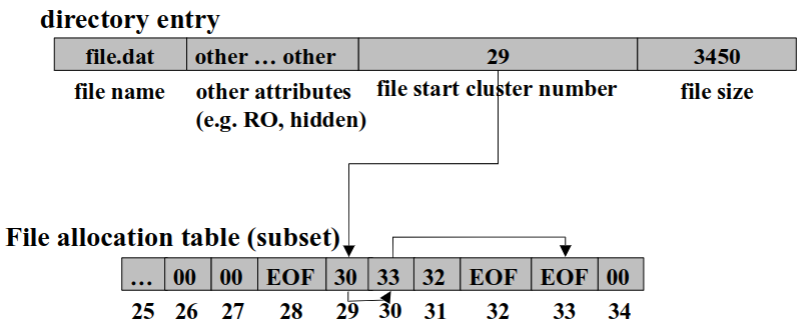
\includegraphics[width=0.8\textwidth]{img/fat.png}
    \caption{Example of a FAT File System Structure}
    \label{fig:fat_file_system}
\end{figure}

\subsubsection{FAT pros and cons}
\begin{itemize}
    \item portability (available to multiple operating systems)
    \item migration (easy switch to richer FS, like NTFS)
    \item fast on small volumes (some GB), due to light "infrastructure (few metadata, no file index, ...)
    \item no integrated advanced features (on-the-fly compression, user quotas)
    \item slow for high numer of files (linked-list structure, fragmentation, no)
    \item no security at all (encryption, access control lists)
\end{itemize}

\section{File Copy and Cloning}

Simple file copy commands preserve file content but may alter file metadata. For forensics, bit-by-bit copies ensure fidelity to the original data, often using the \texttt{dd} command. Variants of \texttt{dd} (e.g., \texttt{dcfldd} and \texttt{dc3dd}) offer additional features like on-the-fly hashing and pattern wiping.

Example commands:
\begin{itemize}
    \item Clone a hard drive to another: \texttt{dd if=/dev/sda of=/dev/sdb}
    \item Create an image file of a hard drive: \texttt{dd if=/dev/hda of=/image.img}
    \item Wipe a drive with binary zeros: \texttt{dcfldd pattern=00 vf=/dev/hdb}
    \item \dots
\end{itemize}

\section{File Identification}

File identification involves determining a file’s actual type and contents, which is crucial in forensics to verify the authenticity and integrity of data. This process often extends beyond simply looking at file extensions, as these are not a reliable source of information.

\begin{itemize}
    \item \textbf{Limitations of Extensions:} File extensions can be easily altered by users or malicious actors, so they should not be solely relied upon to identify a file type.
    \item \textbf{Metadata Inspection:} Whenever possible, examine the file’s metadata, as it often contains information about the file’s true format and origin.
    \item \textbf{File Signatures:} The first few bytes of a file can act as a unique signature, known as a "magic number," which can confirm the file type. A reference list of file signatures can be found online (e.g., \url{https://en.wikipedia.org/wiki/List_of_file_signatures}).
    \item \textbf{Hex Dump Comparison:} By comparing a file's signature with its hex dump, investigators can verify the file type independently of the extension.
\end{itemize}

\section{Metadata Example: File System}

File systems maintain metadata for each file, providing critical information about its content and history. This metadata, managed by the operating system, includes:

\begin{itemize}
    \item \textbf{File Name, Ownership, and Permissions:} Details about the file’s identity, access rights, and owner.
    \item \textbf{Allocated Data Units:} Information on the specific data blocks or clusters assigned to the file.
    \item \textbf{File Size:} The size of the file in bytes.
    \item \textbf{Timestamps:} Key dates associated with the file, such as creation, modification, and last access times.
    \item \textbf{Recovery Data:} Some file systems maintain recovery information (e.g., journaling) that aids in data recovery processes.
\end{itemize}

The type and accuracy of metadata can vary significantly based on the file system in use. Common file systems with differing metadata structures include FAT32, NTFS, ext2, ext3, and ext4.

\section{Slack Space}

Slack space is residual storage within disk sectors allocated to files but not fully utilized. For example, if a 392-byte file is stored in a 512-byte sector, the remaining 120 bytes become slack space, potentially retaining data from prior file storage.

\section{File Recovery Process}

File recovery in forensics involves analyzing file system structures such as the Master File Table (MFT), which stores file metadata, including timestamps. This enables timeline reconstruction, which is crucial for investigating user actions in legal cases. Deleted files, also known as orphan files, may still be recoverable depending on the level of data overwriting and fragmentation.

\section{Metadata Analysis in Files}

Metadata, or "data about data," provides additional insights into file characteristics. Common examples include EXIF metadata for images or embedded metadata in office documents (e.g., DOCX, ODF). Metadata analysis can reveal hidden information, enhance context, and correlate data across files, though it is not inherently trustworthy and may be modified.

\section{Data Sanitization}

Data sanitization tools permanently erase data to prevent unauthorized recovery. Common methods include:
\begin{itemize}
    \item \textbf{File Shredder Programs:} Permanently overwrite selected files.
    \item \textbf{Data Destruction Software:} Fully erases all data on a storage device, useful for secure disposal or virus removal.
\end{itemize}

The Air Force System Security Instruction (AFSSI) 5020 specifies a three-pass overwrite process to ensure data irretrievability.



\end{document}

% Sample of a centered image in LaTeX
% \begin{figure}[h]
%     \centering
%     \includegraphics[width=0.5\textwidth]{path/to/image.png}
%     \caption{Sample Image}
%     \label{fig:sample_image}
% \end{figure}
